\documentclass{beamer}
\usefonttheme{professionalfonts}
\setbeamertemplate{navigation symbols}{}
\usepackage{graphicx}
\usepackage{amsfonts}
\usepackage{amssymb}
\usepackage{takahashi}
\usepackage{xcolor}
\usepackage{subcaption}
\renewcommand\thesubfigure{\arabic{subfigure}}
\definecolor{blue}{rgb}{0.2,0.2,0.7}
\usepackage{tikz}
\usepackage[export]{adjustbox}
\newcommand{\stack}[1]{\begin{tabular}{@{}c@{}}#1\end{tabular}}

\title{Lossless Compression Methods for Archiving Nanopore DNA Signal Data}
\author{
	Sasha Jenner\\
	John Stavrakakis\\
	Ira Deveson\\
	Hasindu Gamaarachchi
}
\institute{B Science and B Adv Studies}
\date{}

\begin{document}
\maketitle

% motivation/objective
\takahashi{
	\frametitle{Motivation}
	\stack{
	Human DNA\\
	\\
	500 000 000 000\\
	data points
	}
}
\takahashi{
	\frametitle{Motivation}
	\stack{
	Walk around Earth\\
	7700 times\\
	\\
	500 000 000 000\\
	steps
	}
}
\takahashi{
	\frametitle{Motivation}
	\stack{
	\begin{columns}
		\begin{column}{0.5\textwidth}
		\centering
		1. Record
		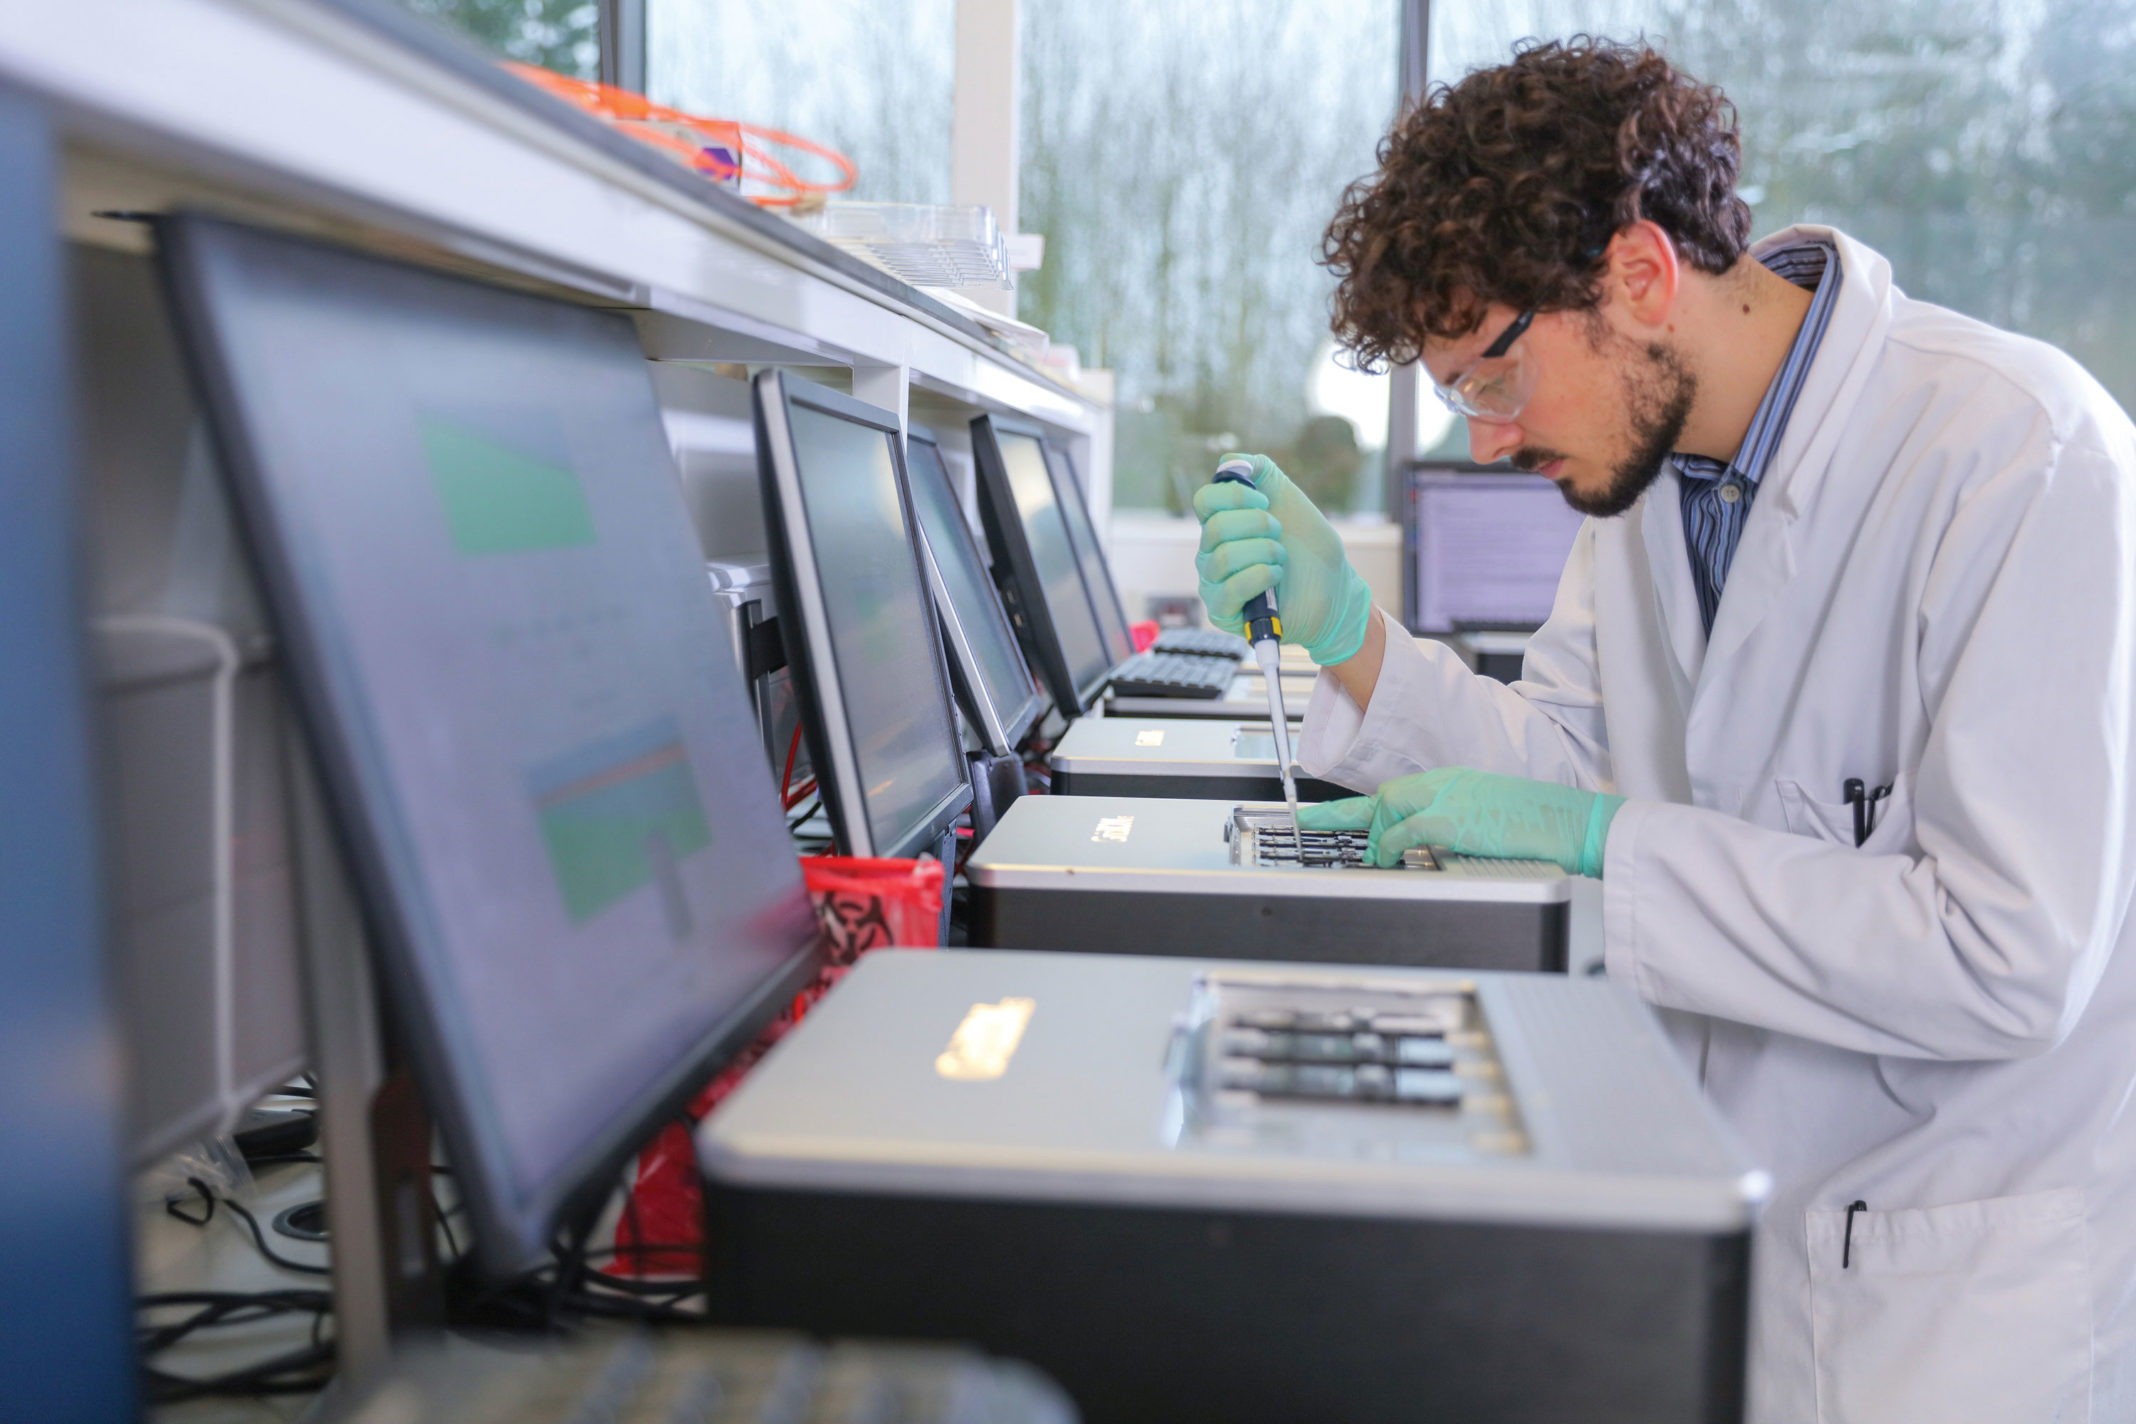
\includegraphics[width=\textwidth]{img/nano-record3.jpg}
		\end{column}
		\begin{column}{0.5\textwidth}
		\centering
		2. Analyse
		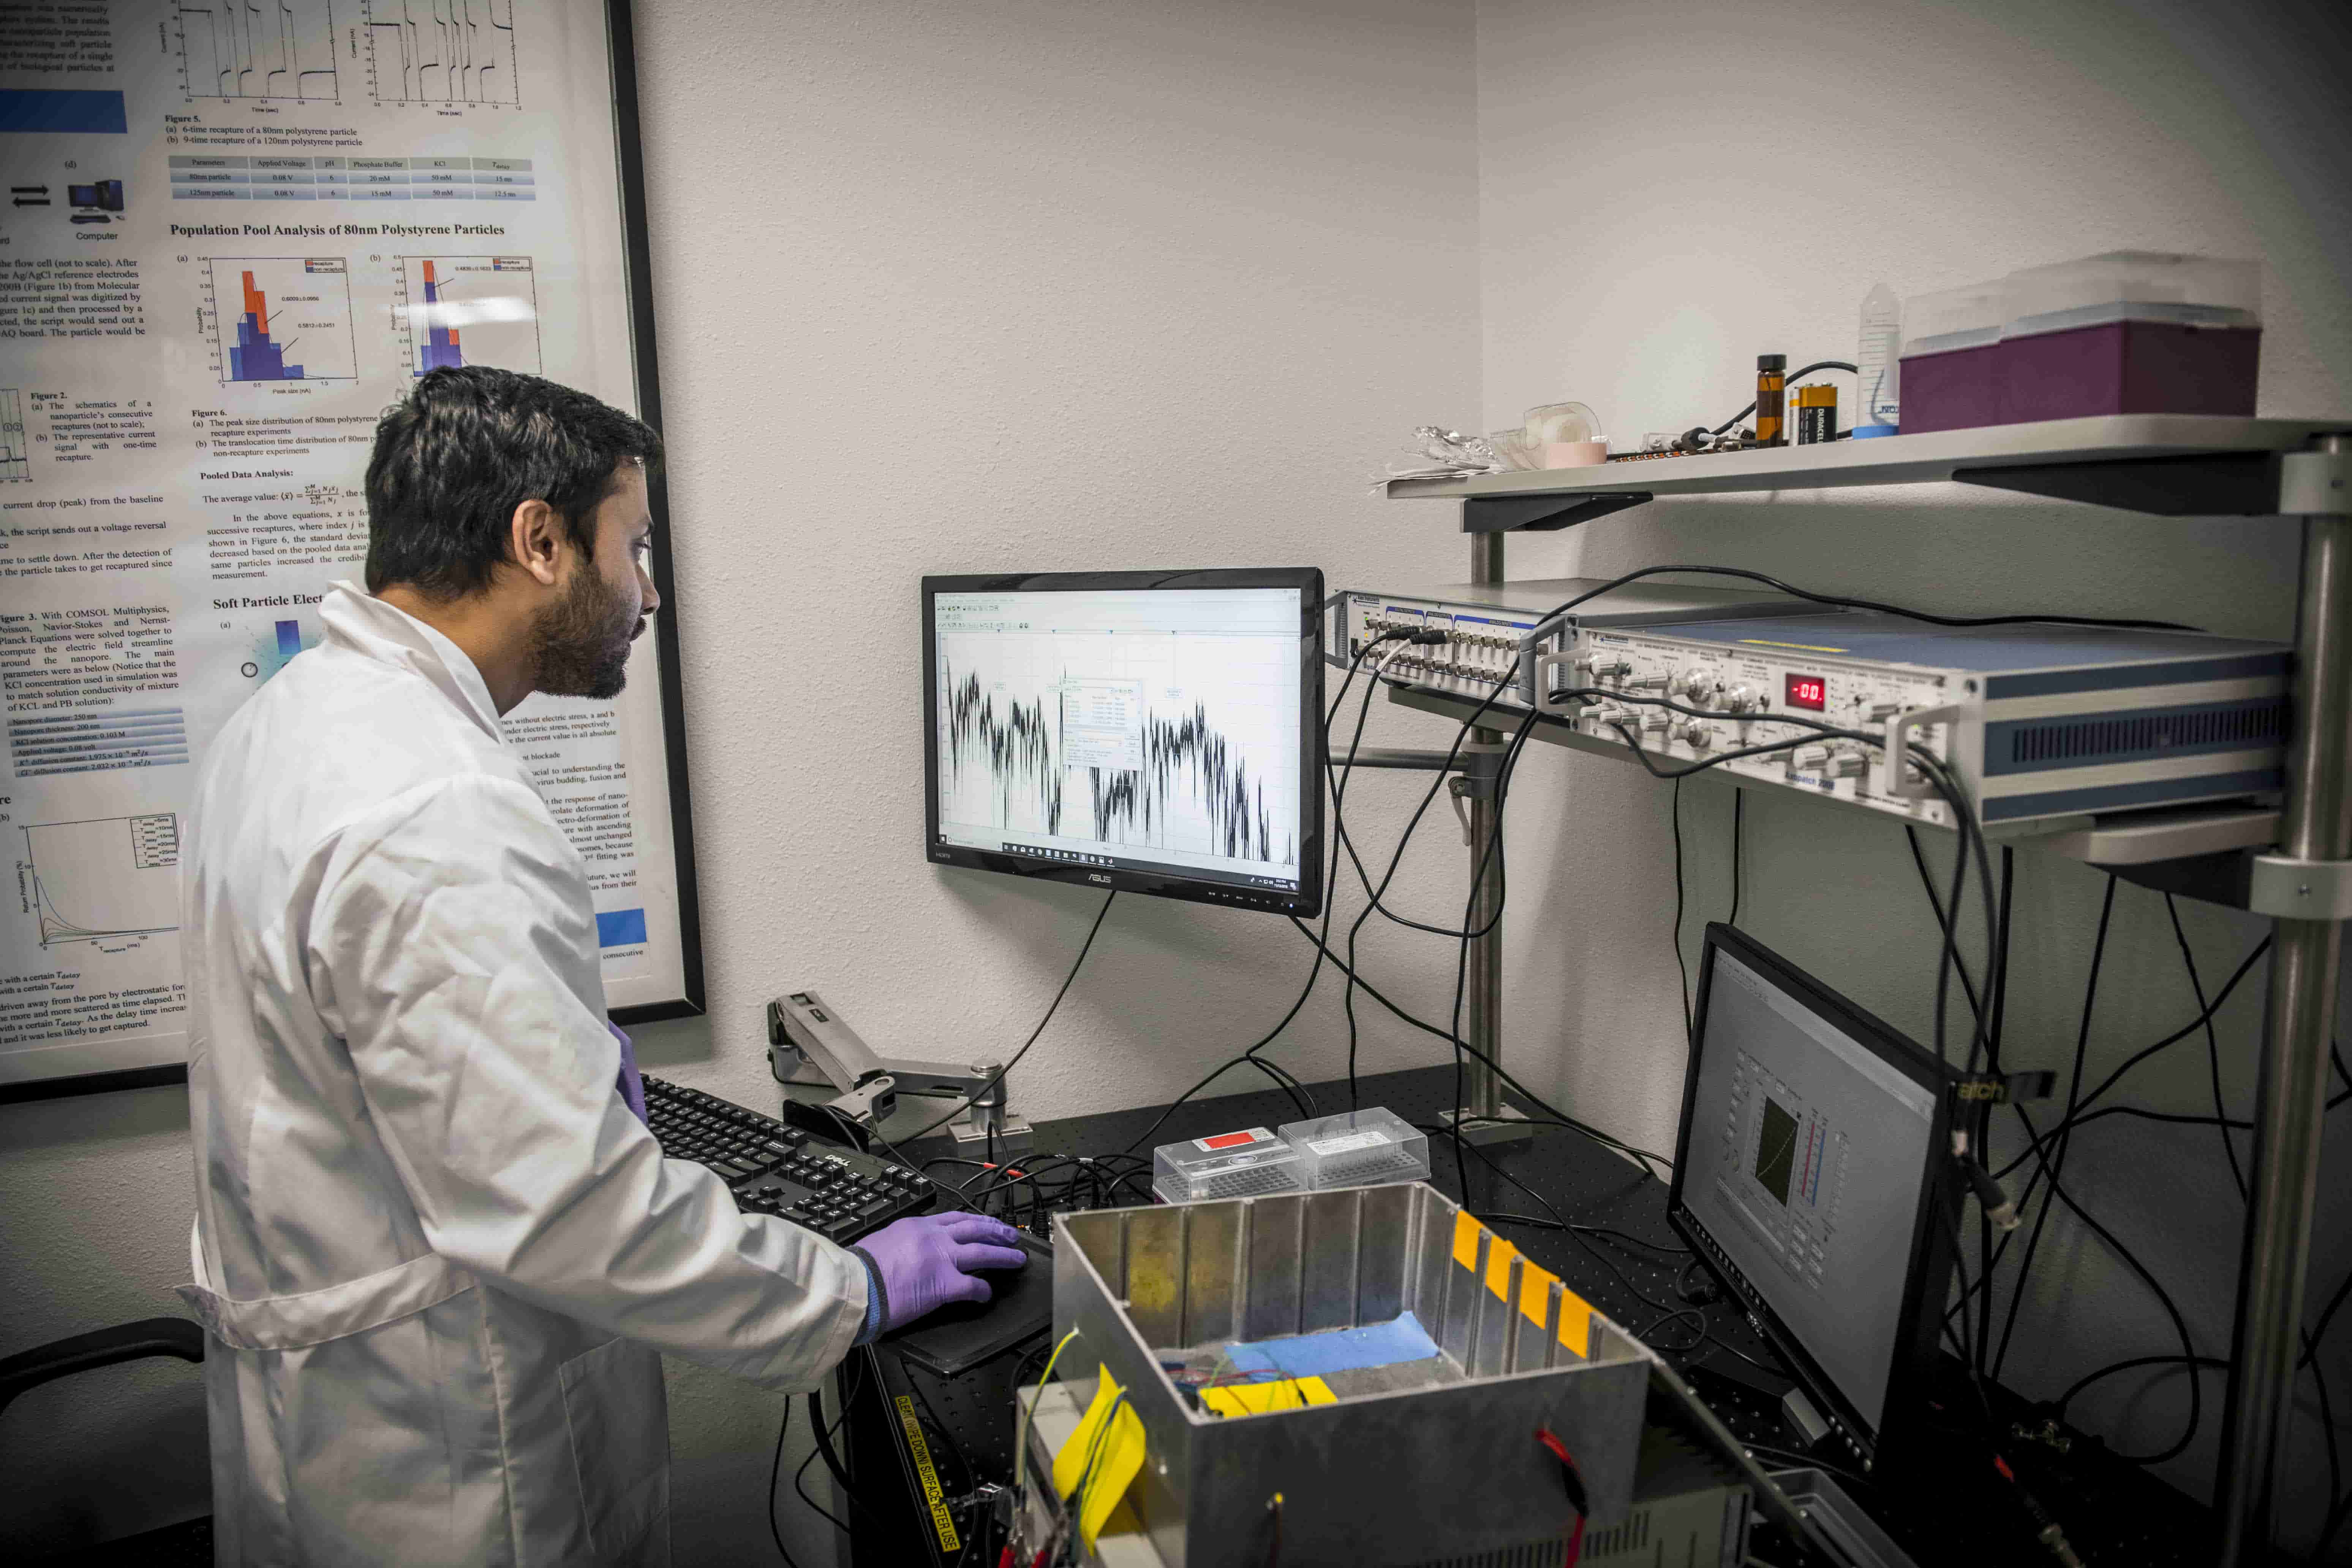
\includegraphics[width=\textwidth]{img/nano-analysis2.jpg}
		\end{column}
	\end{columns}\\
	3. Archive \\
	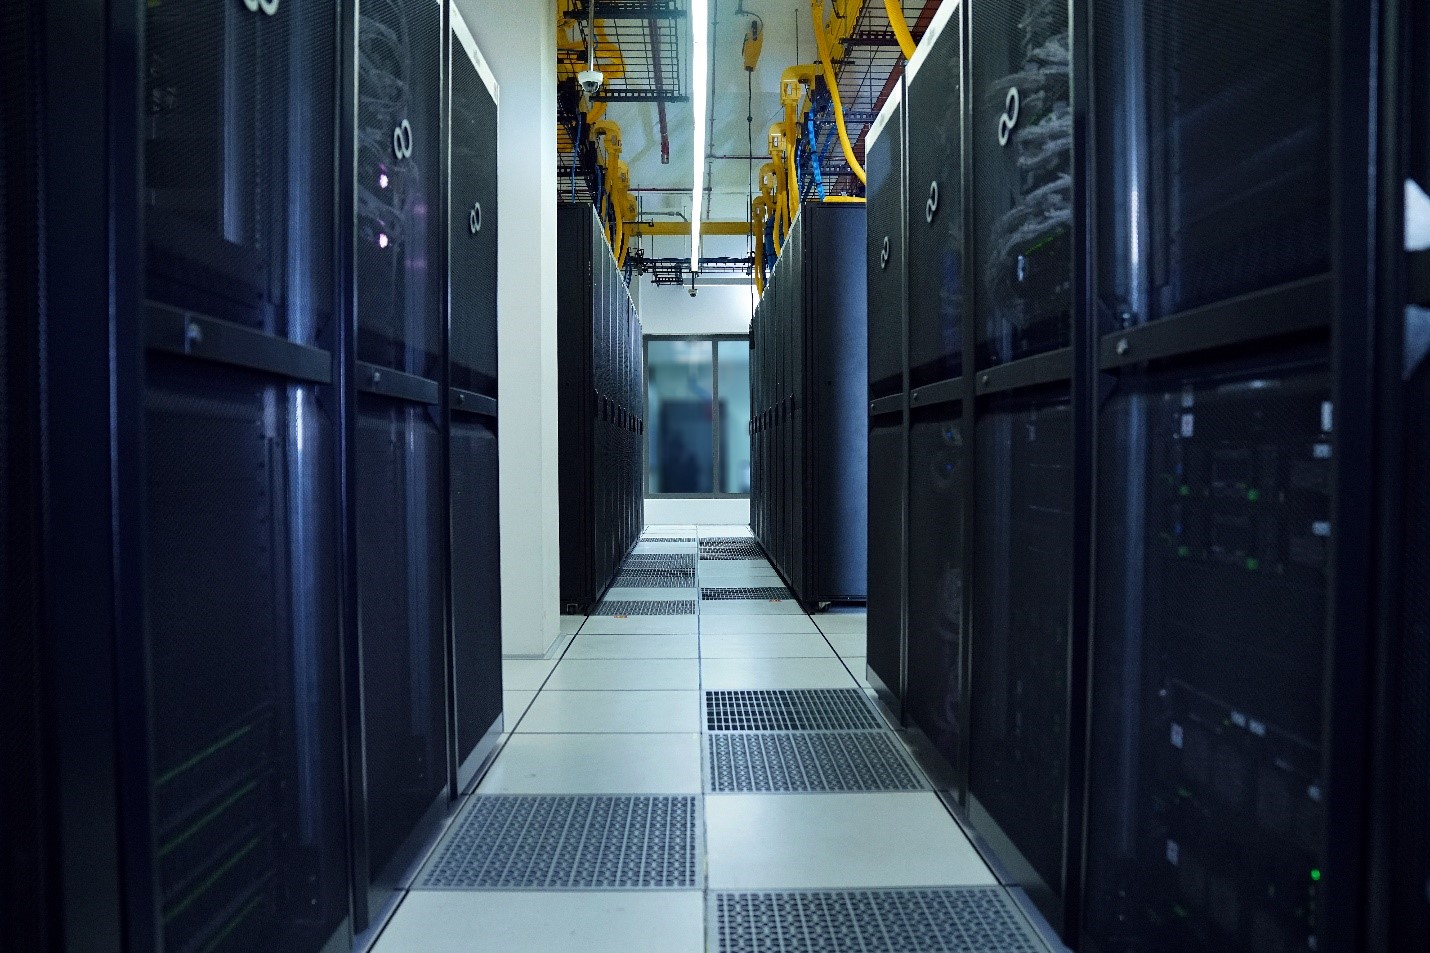
\includegraphics[width=0.5\textwidth]{img/nano-archive3.jpg}
	}
}
%\begin{frame}
%	\frametitle{Motivation}
%	\begin{figure}
%	\begin{subfigure}{0.49\textwidth}
%		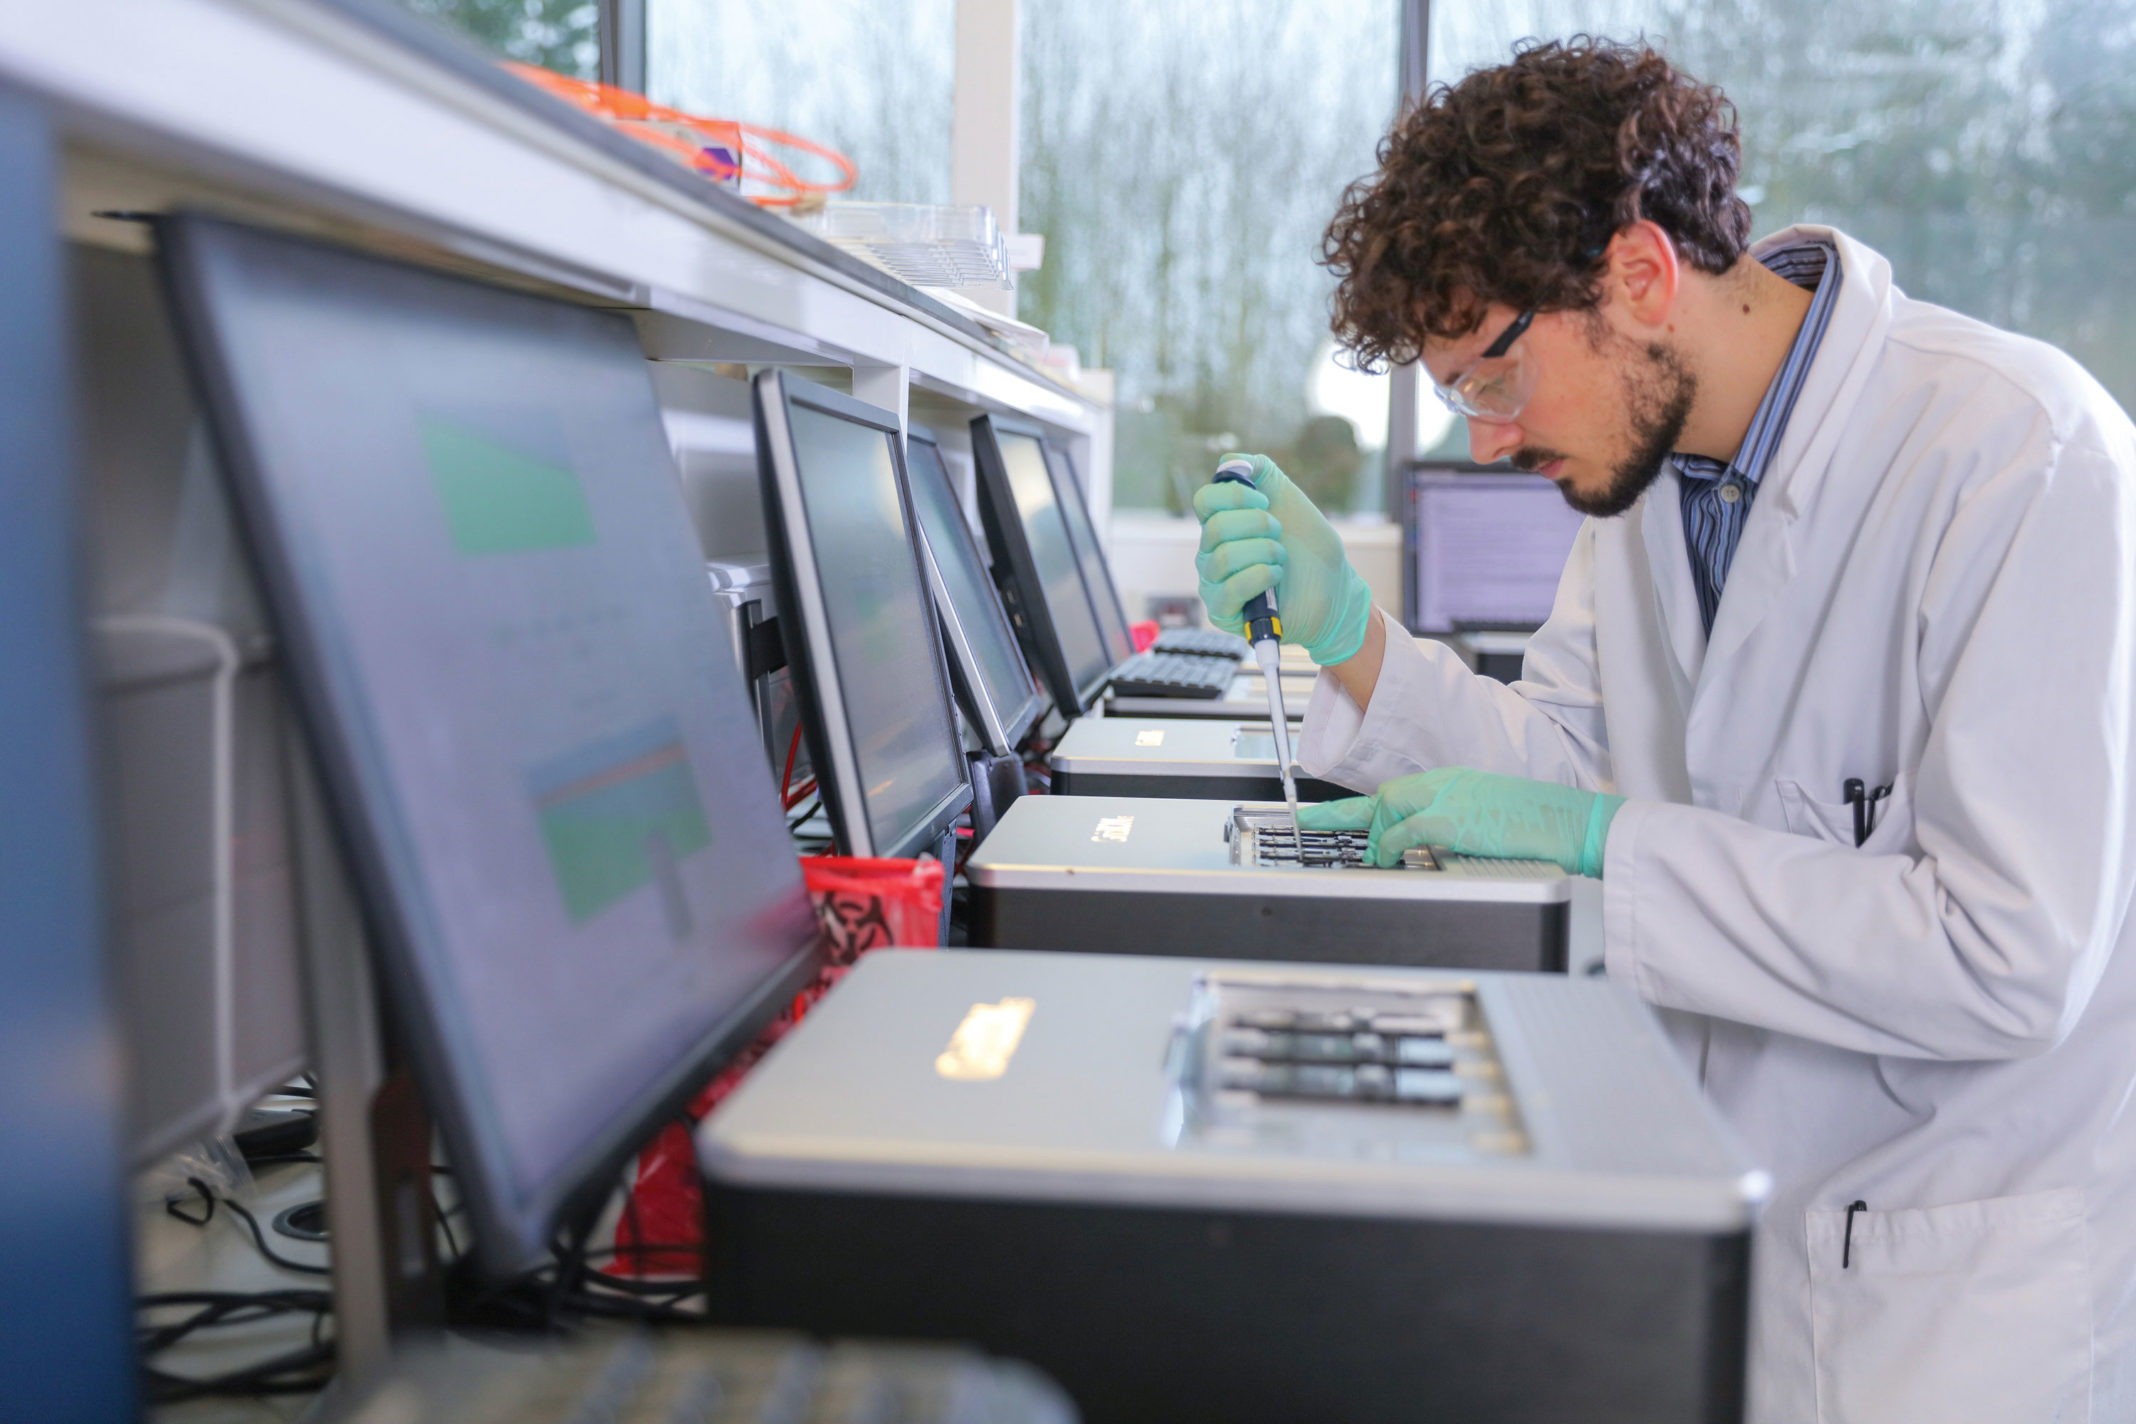
\includegraphics[width=\textwidth]{img/nano-record3.jpg}
%		\caption{Record}
%	\end{subfigure}
%	\hfill
%	\begin{subfigure}{0.49\textwidth}
%		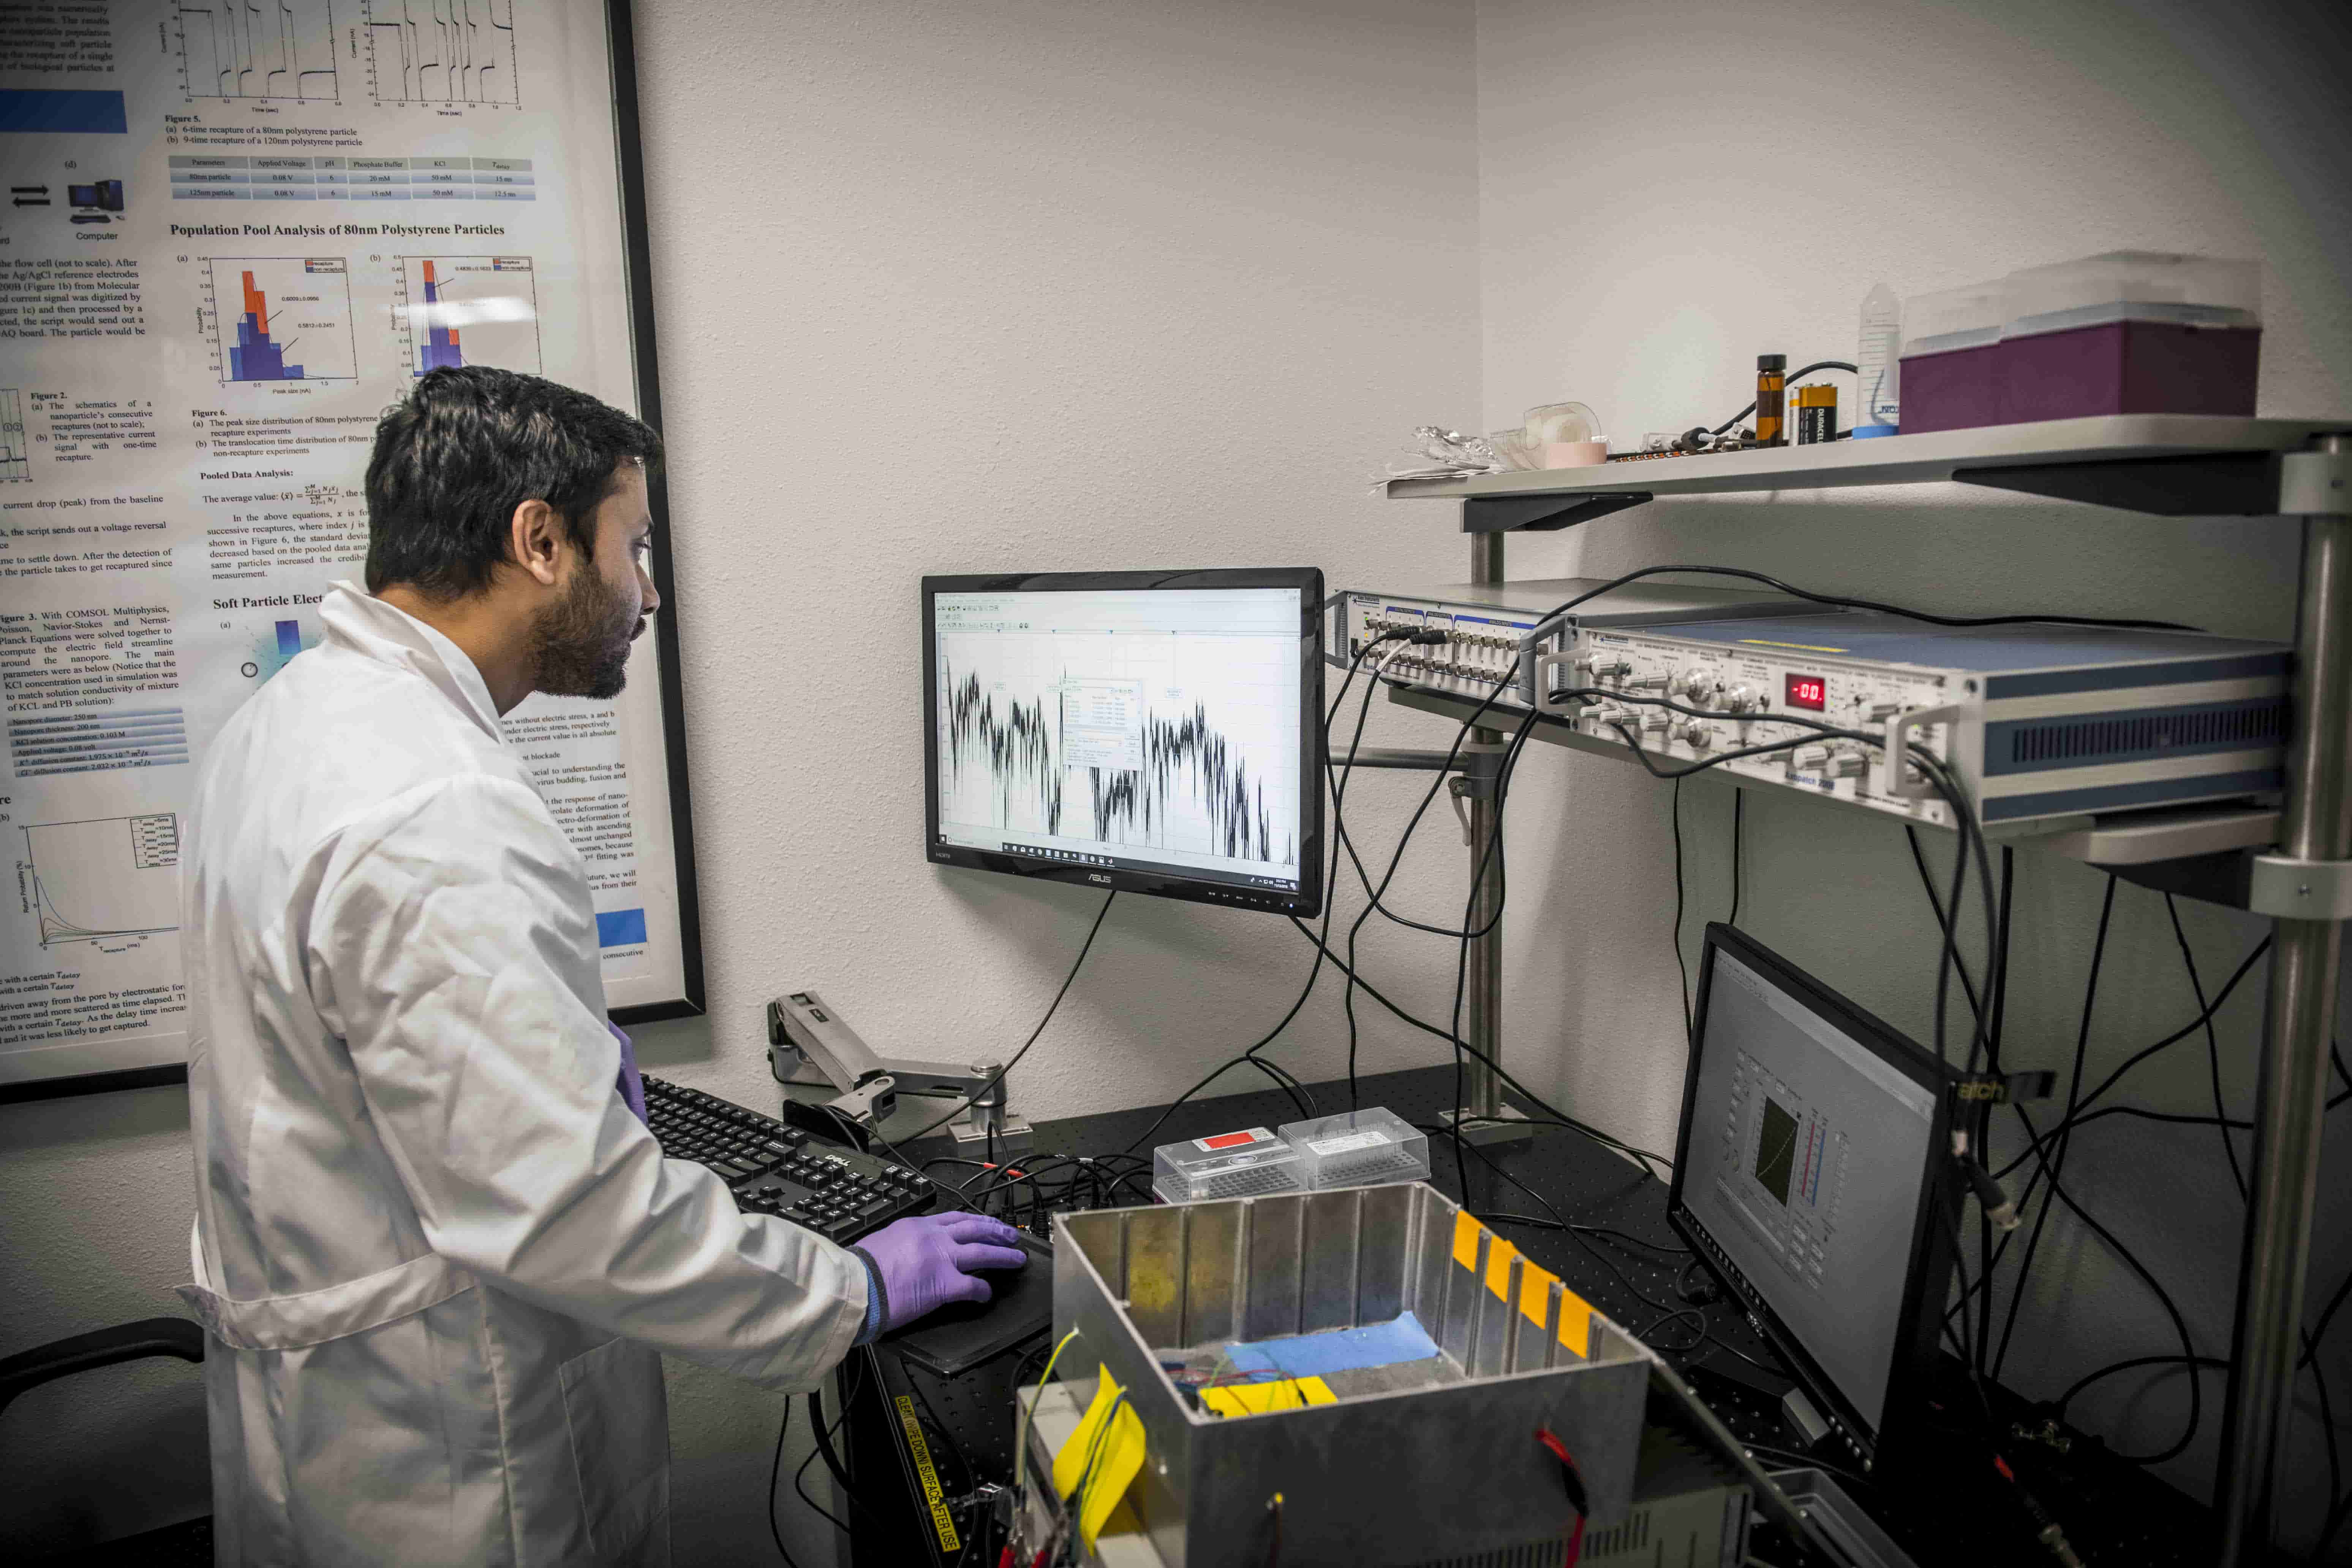
\includegraphics[width=\textwidth]{img/nano-analysis2.jpg}
%		\caption{Analyse}
%	\end{subfigure}
%	\begin{subfigure}{0.49\textwidth}
%		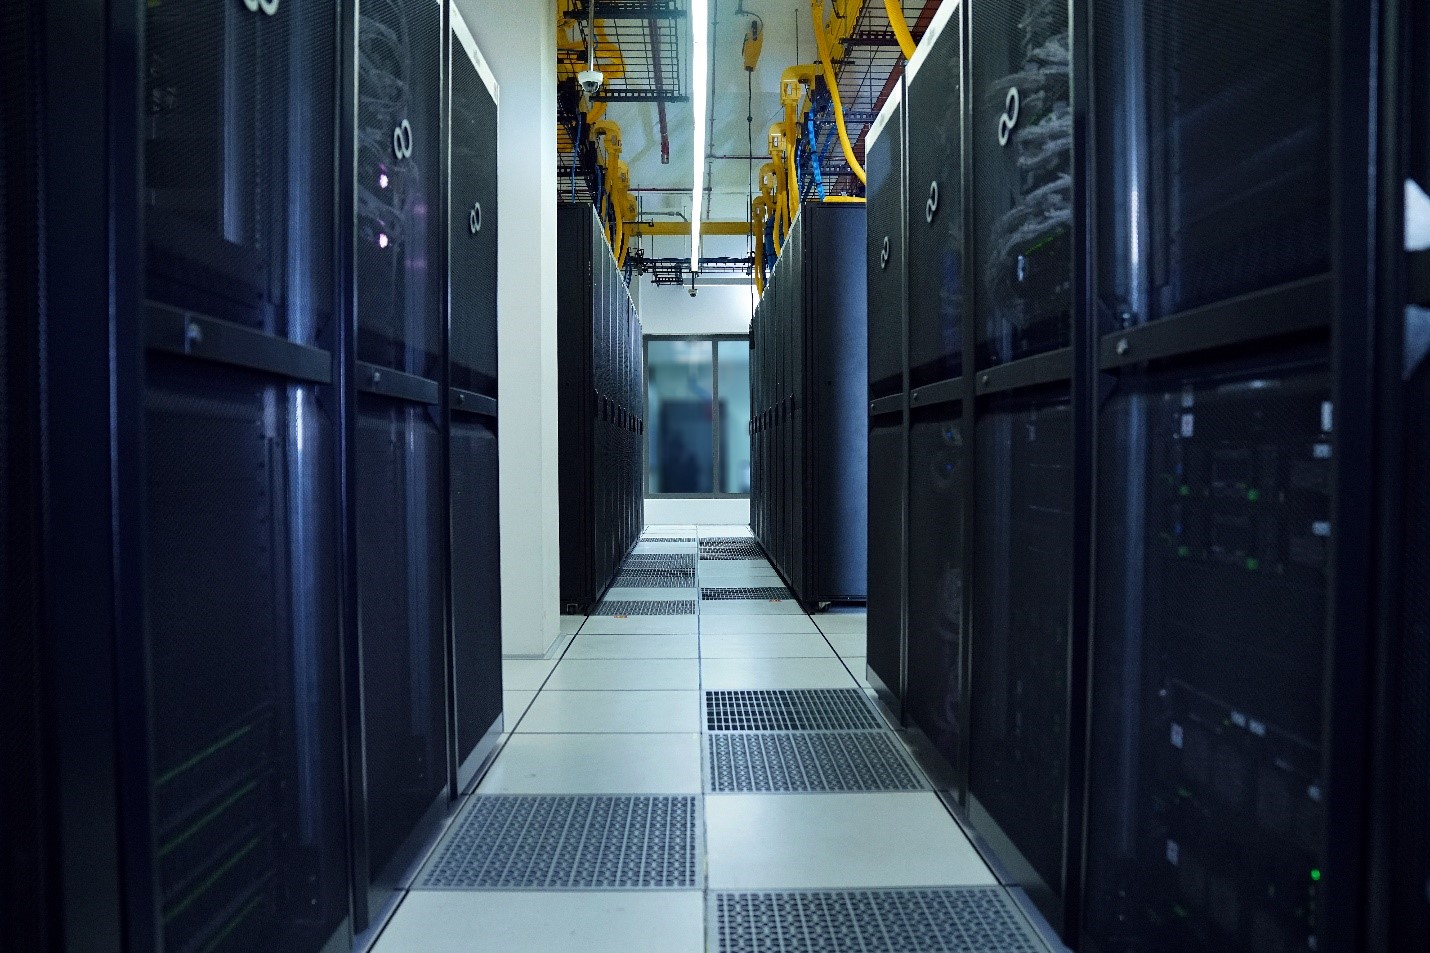
\includegraphics[width=\textwidth]{img/nano-archive3.jpg}
%		\caption{Archive}
%	\end{subfigure}
%	\end{figure}
%\end{frame}
\takahashi{
	\frametitle{Motivation}
	\stack{
	Year 1\\
	\\
	520 terabytes\\
	\$10 000
	}
}
\takahashi{
	\frametitle{Motivation}
	\stack{
	Year 10...\\
	\\
	5 petabytes\\
	\$100 000
	}
}
\takahashi{
	\frametitle{Motivation}
	\stack{
	Data compression\\
	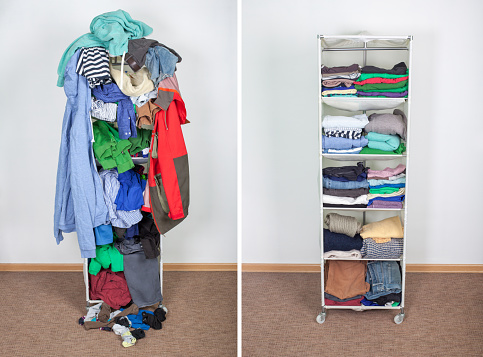
\includegraphics{img/wardrobe.jpg}
	}
}
\takahashi{
	\frametitle{Motivation}
	\stack{
	State-of-the-Art\\
	\\
	Space saving: 65.9\%\\
	Downside: Too generic
	}
}
\takahashi{
	\frametitle{Objective}
	\stack{
	Design compression method\\
	\\
	1. More space saving\\
	2. Suitable for nanopore
	}
}

% background lit
%\takahashi{\color{blue}{Background}}
\takahashi{
	\frametitle{Background}
	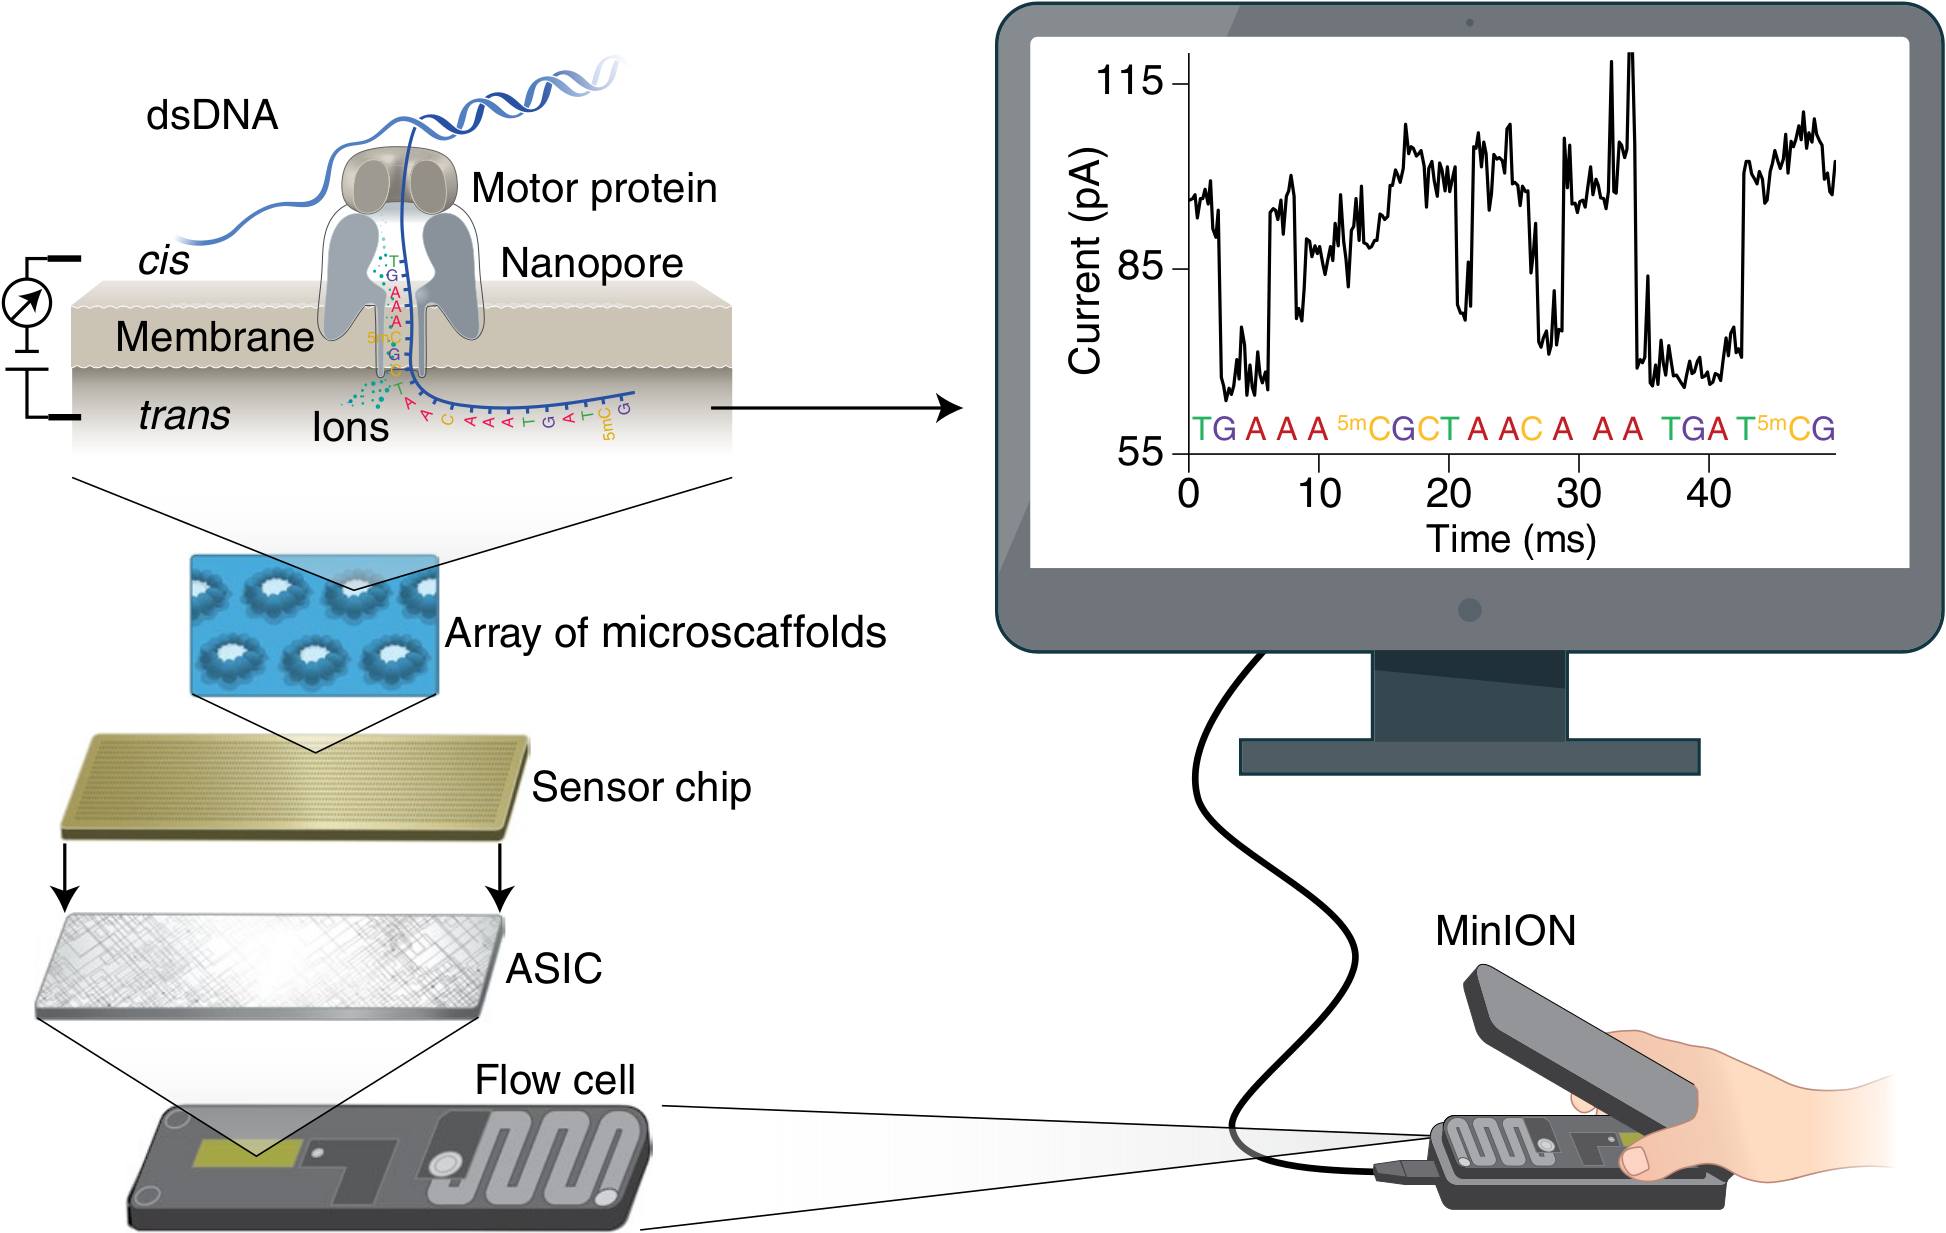
\includegraphics{img/nano.png}
}
\takahashi{
	\frametitle{Background}
	\begin{columns}
		\begin{column}{0.5\textwidth}
		\centering
		Original: 7270K\\
		Lossless: 260K
		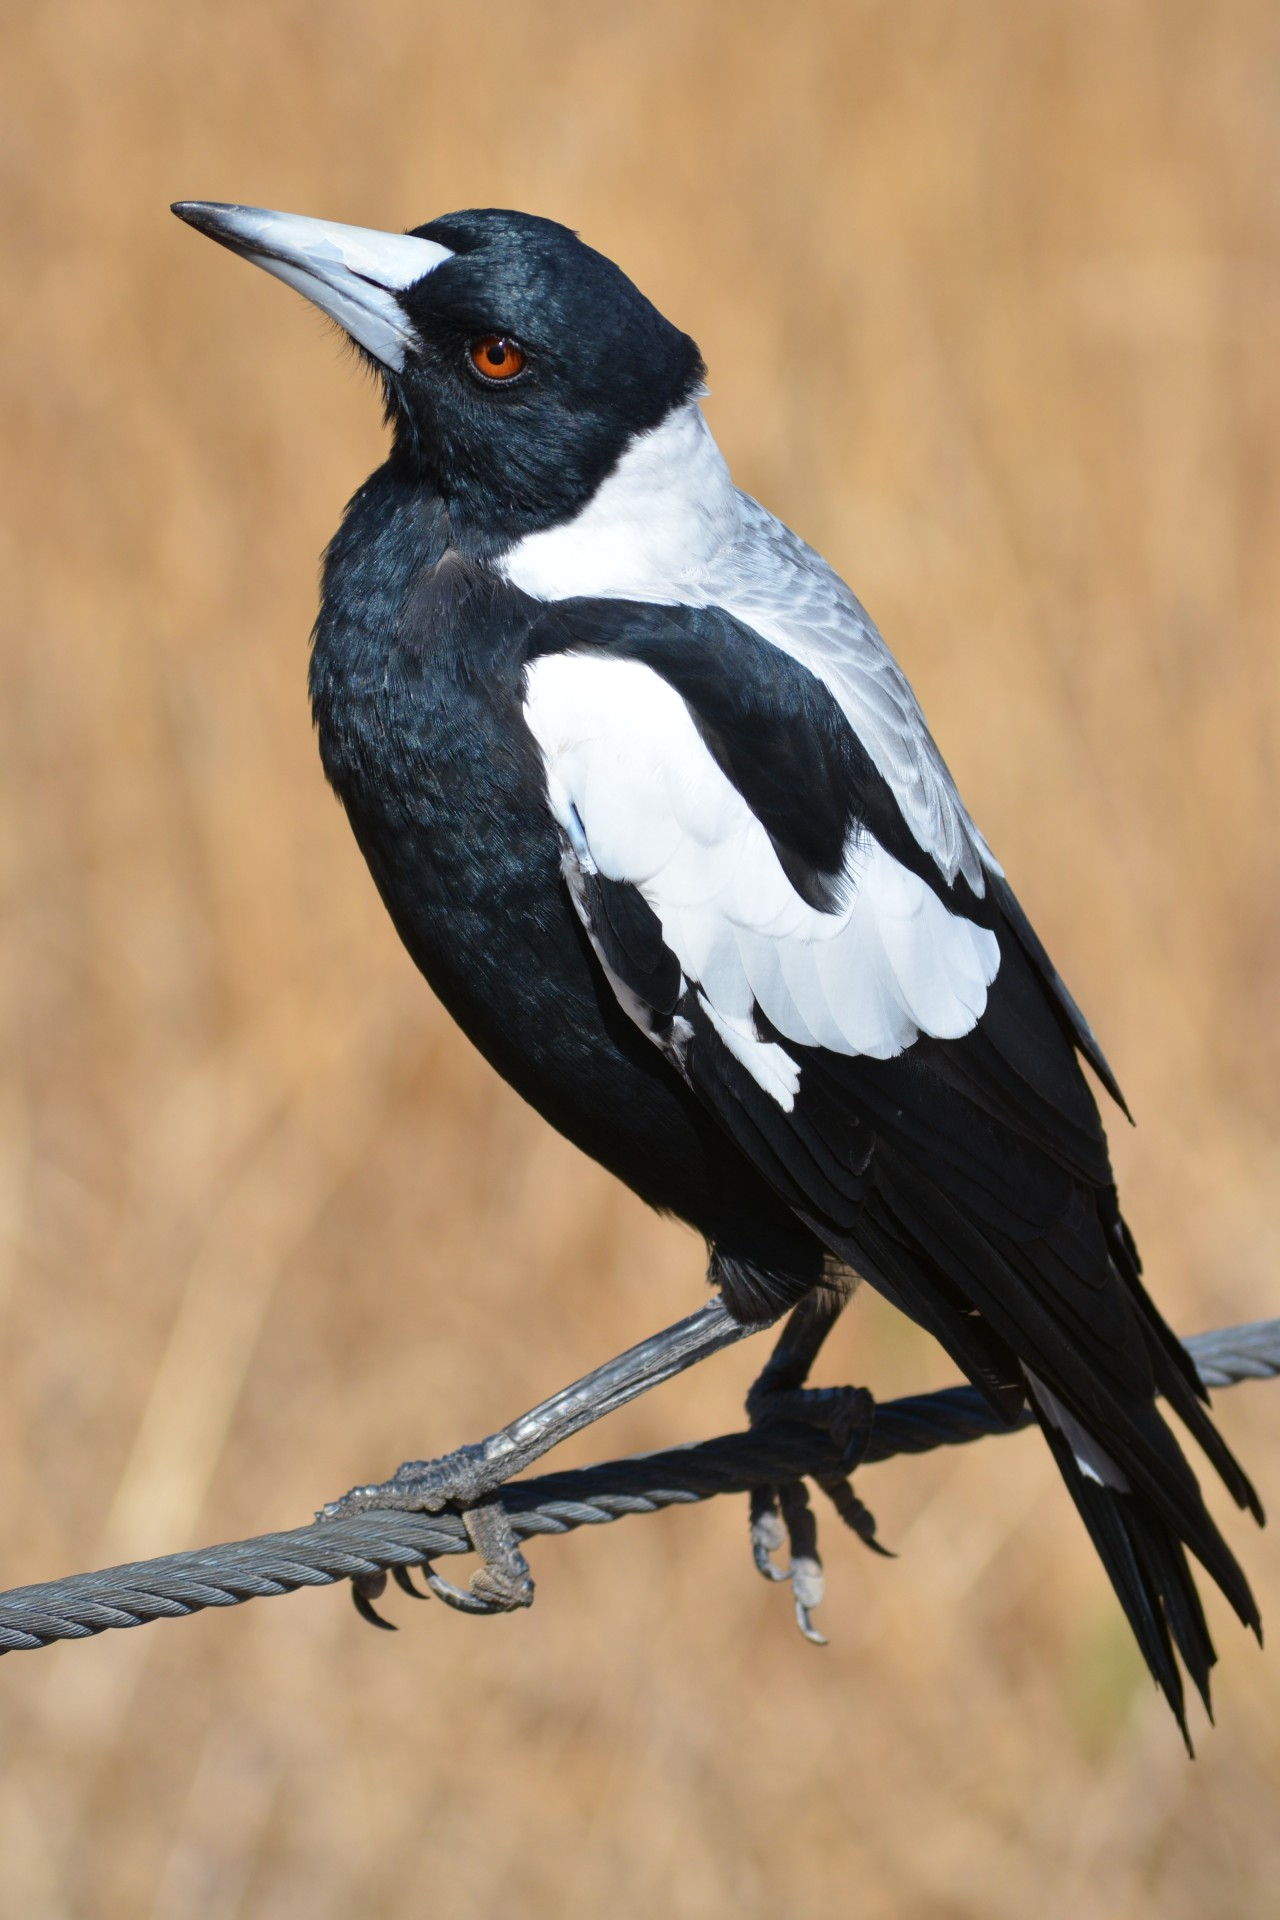
\includegraphics[width=\textwidth]{img/magpie-orig.jpg}
		\end{column}
		\begin{column}{0.5\textwidth}
		\centering
		Lossy: 36K
		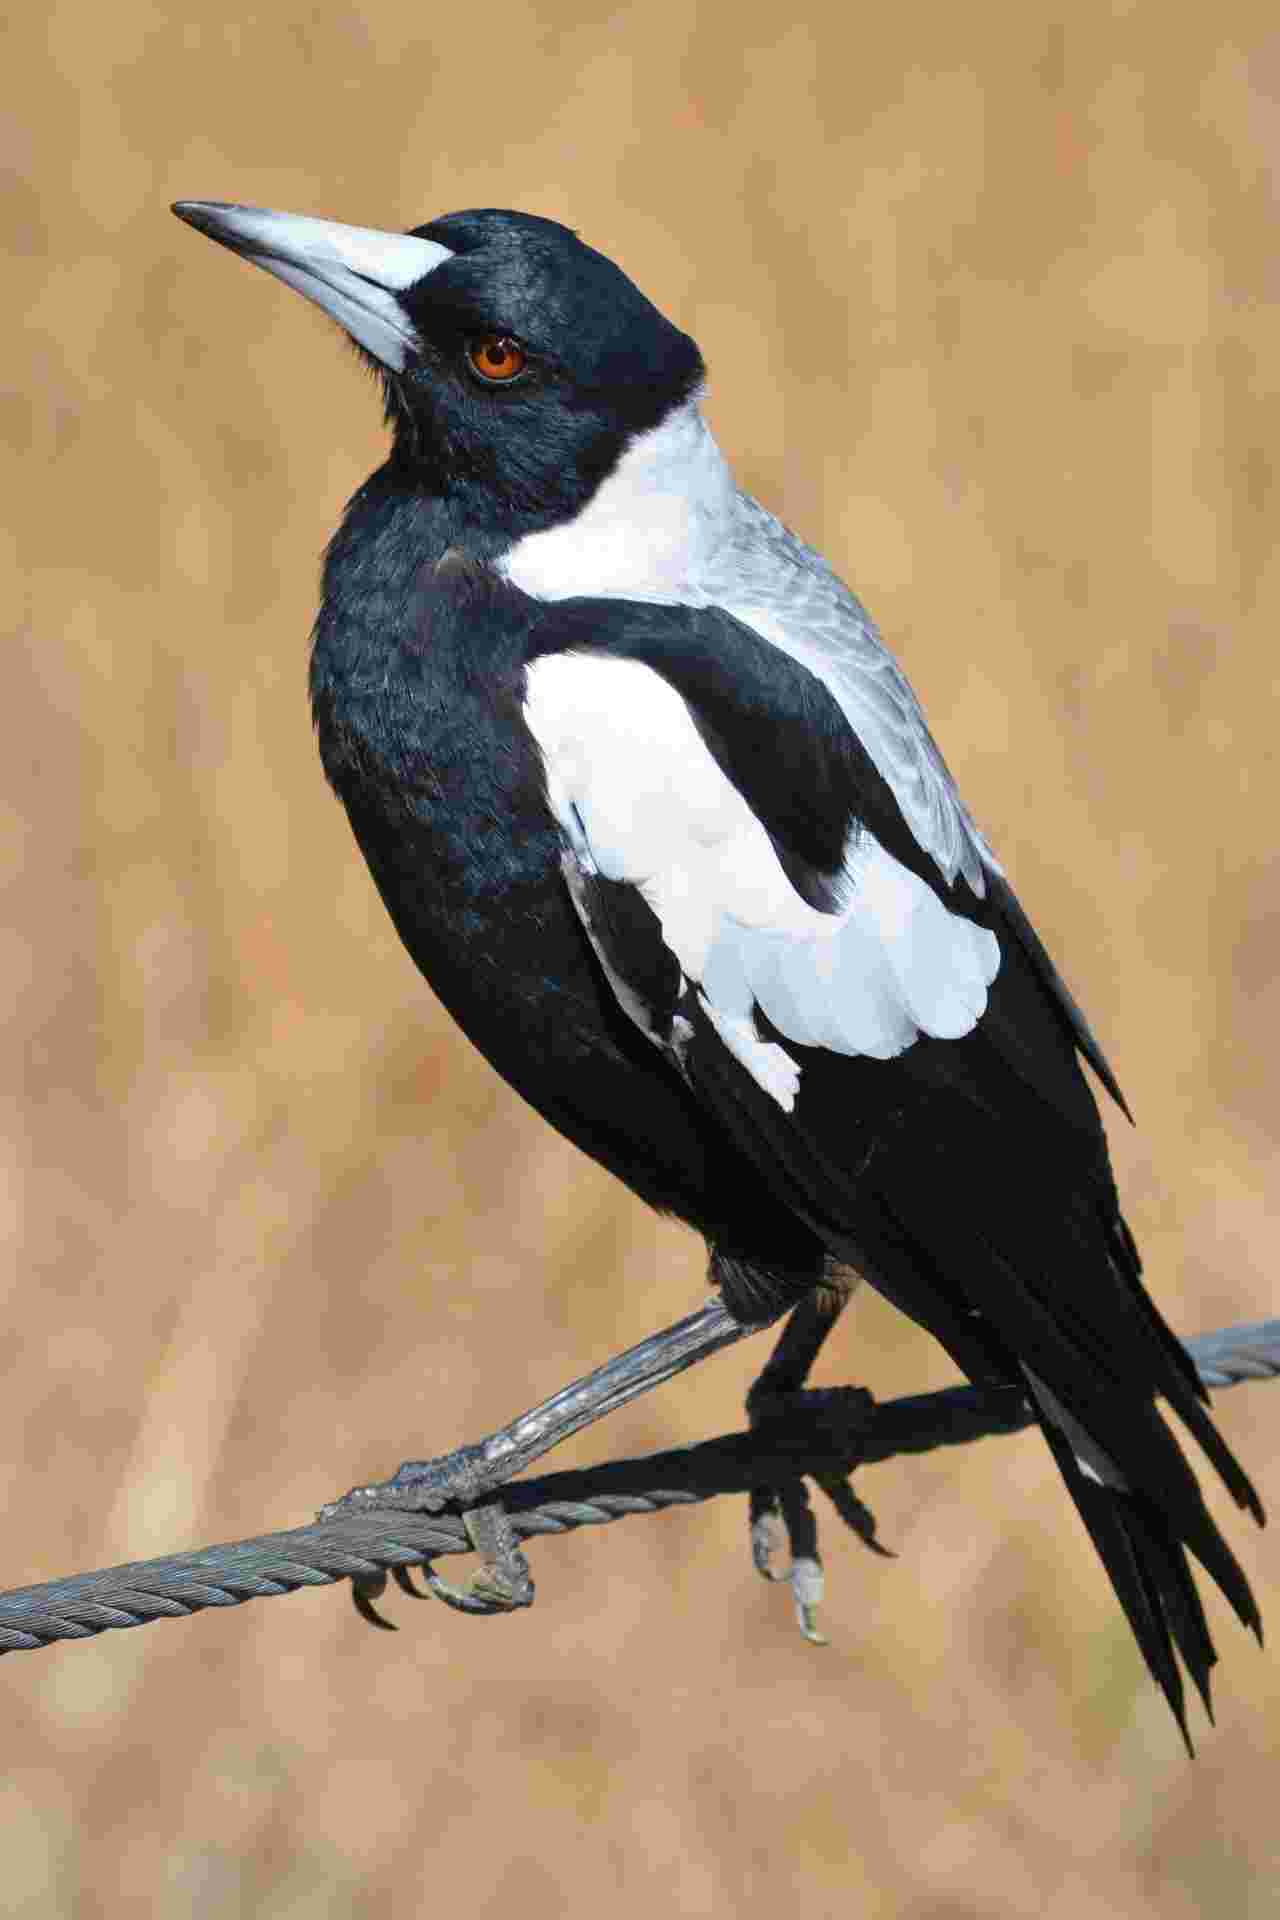
\includegraphics[width=\textwidth]{img/magpie-lossy.jpg}
		\end{column}
	\end{columns}
}
\takahashi{
	\frametitle{Background}
	\stack{
	Entropy $H(X)$: measure of information\\
	\\
	Coin toss: 1 bit\\
	}
}
\takahashi{
	\frametitle{Background}
	\stack{
	Huffman coding
	}
}
%\takahashi{Data compression}
%\takahashi{.mp3, .gz, .zip, .7z}
%\takahashi{How does it work?}
%\takahashi{More frequent = Less bits}
%\takahashi{Huffman coding}
%\takahashi{
%	\stack{
%	AACATTAAAC AATTCAAATG\\
%	TGTGTGCGTC TGTCTGAATT\\
%	CATTTAATTA TTCGTTAATT\\
%	GATTTTCTAC ACAATTAATA\\
%	...}
%}
%\begin{frame}
%	\begin{figure}
%	\begin{adjustbox}{minipage=\linewidth,scale=1.5}
%		\hspace*{2cm}
%	\begin{tabular}{ c|c }
%		Symbol & Code\\
%		A & 00\\
%		C & 01\\
%		G & 10\\
%		T & 11
%	\end{tabular}
%	\end{adjustbox}
%	\end{figure}
%\end{frame}
%\takahashi{
%	\stack{
%	00000100111100000001 00001111010000001110\\
%	11101110111001101101 11101101111000001111\\
%	01001111110000111100 11110110111100001111\\
%	10001111111101110001 00010000111100001100\\
%	...}
%}
%\begin{frame}
%	\begin{columns}[t]
%	\begin{column}{.5\textwidth}
%	\begin{figure}
%	\begin{tabular}{ c|c|c }
%		Symbol & Frequency & Code\\
%		A & 27 & 00\\
%		C & 11 & 010\\
%		G & 9 & 011\\
%		T & 33 & 1
%	\end{tabular}
%	\end{figure}
%	\end{column}
%	\begin{column}{.5\textwidth}
%	\begin{figure}
%	\begin{tikzpicture}
%		\node{80}
%		child {
%			node{57}
%			child {node{A} edge from parent node[left]{0}}
%			child {
%				node{20}
%				child {node{C} edge from parent node[left]{0}}
%				child {node{G} edge from parent node[right]{1}}
%				 edge from parent node[right]{1}
%			}
%			edge from parent node[left]{0}
%		}
%		child {node{T} edge from parent node[right]{1}};
%	\end{tikzpicture}
%	\end{figure}
%	\end{column}
%	\end{columns}
%\end{frame}
%\takahashi{
%	\stack{
%	00000100011000000010 0000110100000001011\\
%	1011101110110100111010 101110101011000011\\
%	0100011100001100 1101001111000011\\
%	011001111010100010 000100000110000100\\
%	...}
%}
%\takahashi{Compression Ratio = $\frac{2\times 80 bits}{147 bits} \approx 1.1$}
%\takahashi{gzip}
%%\begin{frame}
%%	\includegraphics[scale=1]{gzip.png}
%%\end{frame}
%\takahashi{VBZ}
%\takahashi{
%	\stack{
%	Integer sequence\\
%	Differences\\
%	Map to unsigned\\
%	Stream VByte\\
%	Zstandard}
%}
%% TODO scale up
%%\begin{frame}
%%	\begin{enumerate}
%%	\item Integer sequence
%%	\item Differences
%%	\item Map to unsigned
%%	\item Stream VByte
%%	\item Zstandard
%%	\end{enumerate}
%%\end{frame}
%\takahashi{
%	\frametitle{Integer sequence}
%	\stack{
%	1039,588,588,593,586,\\
%	574,570,585,588,586,\\
%	578,582,584,586,597,\\
%	...}
%}
%\takahashi{
%	\frametitle{Differences}
%	\stack{
%	1039,-451,0,5,-7,\\
%	-12,-4,15,3,-2,\\
%	-8,4,2,2,11,\\
%	...}
%}
%\takahashi{
%	\frametitle{Map to unsigned}
%	\stack{
%	2078,901,0,10,13,\\
%	23,7,30,6,3,\\
%	15,8,4,4,22,\\
%	...}
%}
%\takahashi{
%	\frametitle{Stream VByte}
%	\stack{
%	10|10|00|01|01|\\
%	01|01|01|01|01|\\
%	01|01|01|01|01|\\
%	...\\
%	0x1e 0x08|0x85 0x03||0x0a|0x0d|\\
%	0x17|0x07|0x1e|0x06|0x03|\\
%	0x0f|0x08|0x04|0x04|0x16|\\
%	...}
%}
%\takahashi{Zstandard}

% method
%\takahashi{\color{blue}{Research Method}}
%\takahashi{1. Determine the features of the data}
%\takahashi{2. Experiment with existing encoders}
%\takahashi{3. Develop a better lossless encoder}
%\takahashi{(a) Higher best compression ratio}
%\takahashi{
%	\stack{
%	(b) Higher compression-time ratio\\
%	$=\frac{\text{compression ratio}}{\text{time taken}}$}
%}

% results
%\takahashi{\color{blue}{Plan}}
%\begin{frame}
%	\begin{figure}
%	\begin{adjustbox}{minipage=\linewidth,scale=1.5}
%	\begin{tabular}{c|c}
%		Task & Timeline\\
%		Data features & 8/3 -- 15/6\\
%		Encoding experiments & 10/5 -- 1/10 \\
%		Develop new encoder & 1/8 -- 1/10 \\
%		Test encoder & 12/9 -- 17/10 \\
%		Thesis & Sep -- Nov\\
%		Presentation & Oct -- Nov
%	\end{tabular}
%	\end{adjustbox}
%	\end{figure}
%\end{frame}

% discussion/evaluation/contribution

% conclusion/future work

% questions
\takahashi{Questions?}

\end{document}
